\documentclass[10pt,a4paper]{article}

\usepackage[T1]{fontenc}
\usepackage[polish]{babel}
\usepackage[utf8]{inputenc}
\usepackage{graphicx}
\usepackage[export]{adjustbox}

\graphicspath{ {./../../media/} }

\usepackage[margin=1.2in]{geometry}

\usepackage{hyperref}
\hypersetup{
    colorlinks=true,
    linkcolor=black,
    filecolor=magenta,      
    urlcolor=blue,
}

\usepackage{amsfonts}
\usepackage{titlesec}

\titleformat{\chapter}[hang] 
{\normalfont\huge\bfseries}{\chaptertitlename\ \thechapter:}{1em}{} 
\titleformat*{\section}{\huge}
\begin{document}

\title{\Huge Dokumentacja migracji na środowisko linux.}
\author{Maciej Tracz \\\\Technikum Mechatroniczne nr 1 w Warszawie}
\date{Rok 2020}
\maketitle

\textbf{Uwaga!} \textbf{Proces instalowania wymaga operacji na dyskach twardych twojej maszyny. Może to wiązać się to z omyłkowym usunięciem danych lub ich zniszczeniem. Przez rozpoczęciem upewnij się, że masz zrobioną kopię zapasową wszystkich ważnych plików i/lub poprzedniego systemu operacyjnego.}

	\section{Instalacja}
	
Proces instalowania warto podzielić na 3 etapy:
\begin{enumerate}
\item Tworzenie nośnika ISO
\item Instalacja systemu na docelowej maszynie
\item Konfiguracja poinstalacyjna\\
\end{enumerate}	
Teraz kolejno przejdziemy przez wszystkie 3 na przykładzie Linux Manjaro XFCE 20.0.3.
		\subsection{Tworzenie nośnika}
Aby móc zainstalować system operacyjny na komputerze potrzebujemy urządzenia będącego nośnikiem obrazu takiego systemu. Do tego potrzebujemy pendriva conajmniej 8GB oraz obrazu systemu w postaci ISO. Taki można pobrać na stronach twórców w zakładce Downloads. Gdy mamy już te elementy potrzebujemy narzędzia, które przygotuje pendriva jako nośnik. Polecam Rufusa dla użytkowników Windowsa oraz UUByte Software na MacOS. Nie są to jednak jedyne opcje i warto poszukać czy aktualnie nie wyszły nowsze, lepsze narzędzia.\\\\Windows\\\\Rufus: \url{https://rufus.ie/}\\ YUMI: \url{https://www.pendrivelinux.com/yumi-multiboot-usb-creator/}\\\\MacOS\\\\\ UUByte Software: \url{https://www.uubyte.com/download/uubyte-iso-editor.dmg}\\Disk Utility - The Default ISO Buner (narzędzie wbudowane, polecane na starych urządzeniach.)\\\\\\ Teraz gdy masz masz wszytsko co potrzebne, postępuj zgodnie z instrukcją na stronie lub po prostu dodaj ISO i wybierz domyślne ustawienia. Jeśli posiadasz już odpowiednio przygotowanego pendriva przejdzmy do następnego etapu.
		
		\subsection{Instalacja}
		
Przedstawię tutaj przykładową instalację Linuxa Manjaro w najnowszej dla mnie wersji. Wiele elementów bedzie niezmienna w przypadku wiekszości dystrybucji. Jednak jeśli nie jesteś pewien swoich umiejętności adaptacji zachęcam do poszukanie w internecie poradników przystosowanych do twoich potrzeb.

\begin{enumerate}
\item \textbf{Wybór urządzenia do rozruchu.}\par
Po włożeniu pendriva do komputera, aby go wybrać, trzeba tą maszynę uruchomić ponownie i podczas uruchamiania klikać przycisk F9, F10 lub F12 zależnie od producenta. Taką informację łatwo znaleźć szukając frazy "boot key [nazwa producenta lub model]". Gdy już uda nam się przejść do manu wyboru, wybieramy nasz pendrive i czekamy aż obraz się załaduje.\\

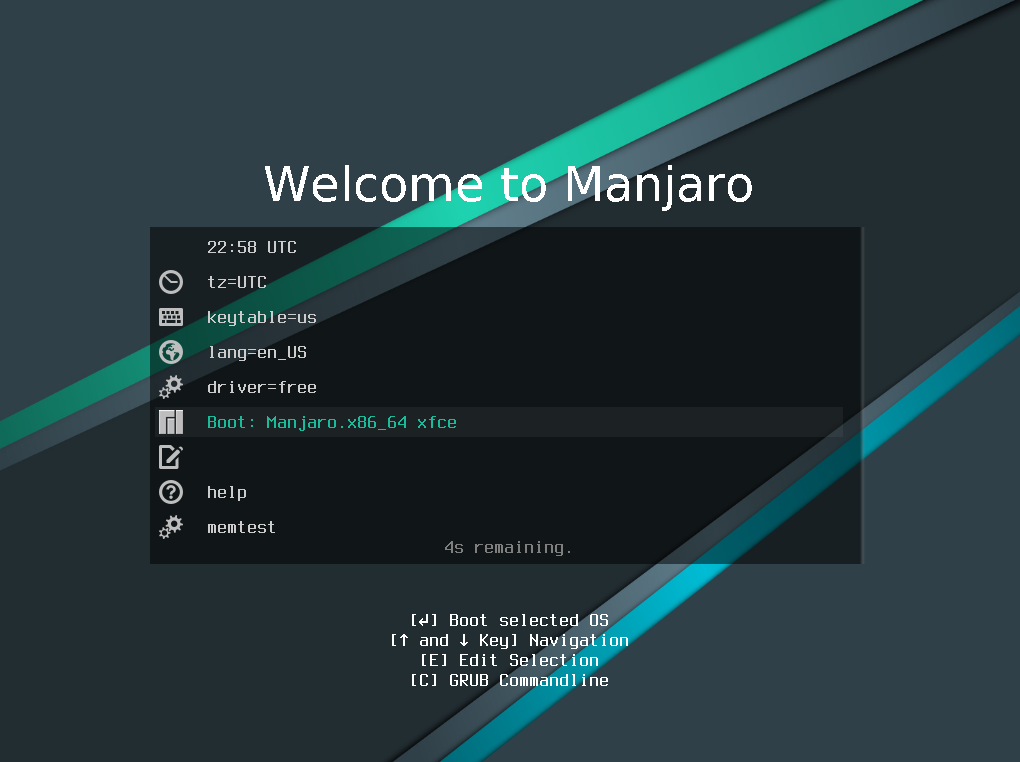
\includegraphics[width=0.6\textwidth, center]{manjaro_install1.png}

\item \textbf{Live USB} \par
W tym momencie jesteśmy w środku środowiska instalacyjnego. Możemy tu sprawdzić jak wizualnie będzie wyglądał system, jakie będziemy mieli opcje konfiguracji czy też jak nam się używa taki interfejs. Gdy już skończysz oględziny i uznamy, że chcemy kontynuować wybieramy instalator z pulpitu i przechodzimy dalej.\\

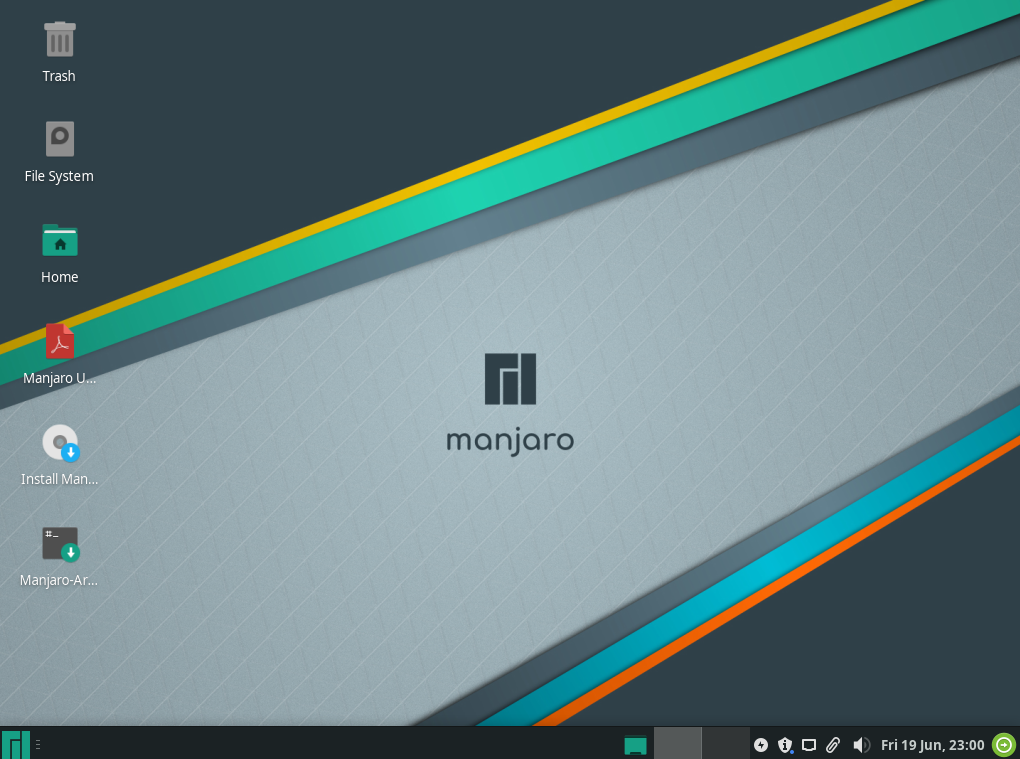
\includegraphics[width=0.75\textwidth, center]{manjaro_install2.png}



\item \textbf{Instalator} \par
Wiele dystrybucji posiada polskie instalatory co ułatwi proces osobą z mniejszym zrozumieniem języka angielskiego. Każdy też ma swoje specyficzne etapy, które charakteryzują różne dystrybucje.\\

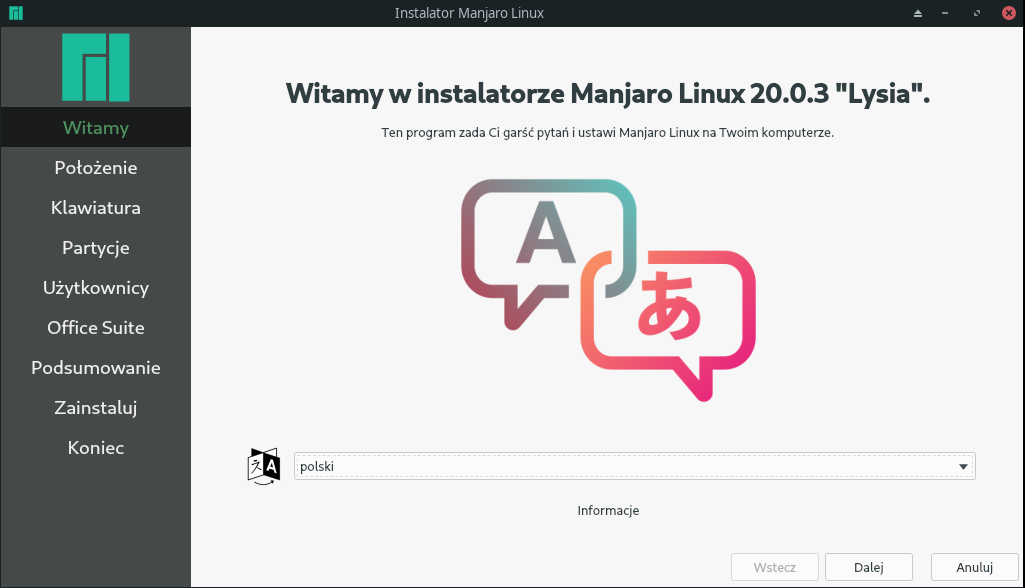
\includegraphics[width=0.95\textwidth, center]{manjaro_install3.png}\\\\\\

\item \textbf{Wybór strefy czasowej} \par
Aby upewnić się, że czas systemowy jest taki sam jak czas na twoim zegarku musimy ustawić strefę czasową dla servera NTP.\\

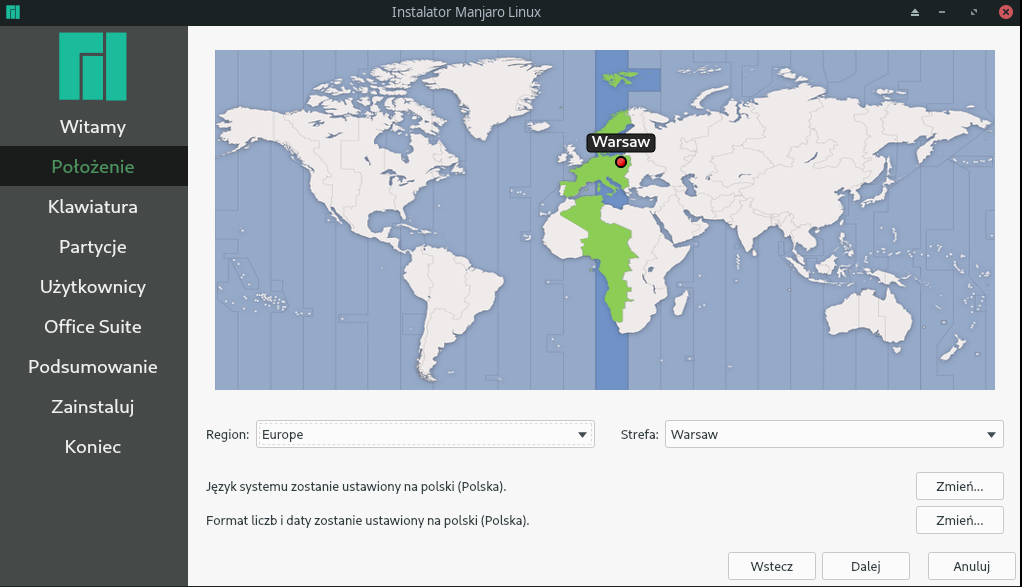
\includegraphics[width=0.95\textwidth, center]{manjaro_install4.png}\\\\\\



\item \textbf{Klawiatura} \par
Jeśli masz w imieniu lub po prostu zamierzasz użyć polskich znaków lub innych niedostępnych na standardowej klawiaturze angielskiej, wybierz układ odpowiedni do twoich potrzeb.\\

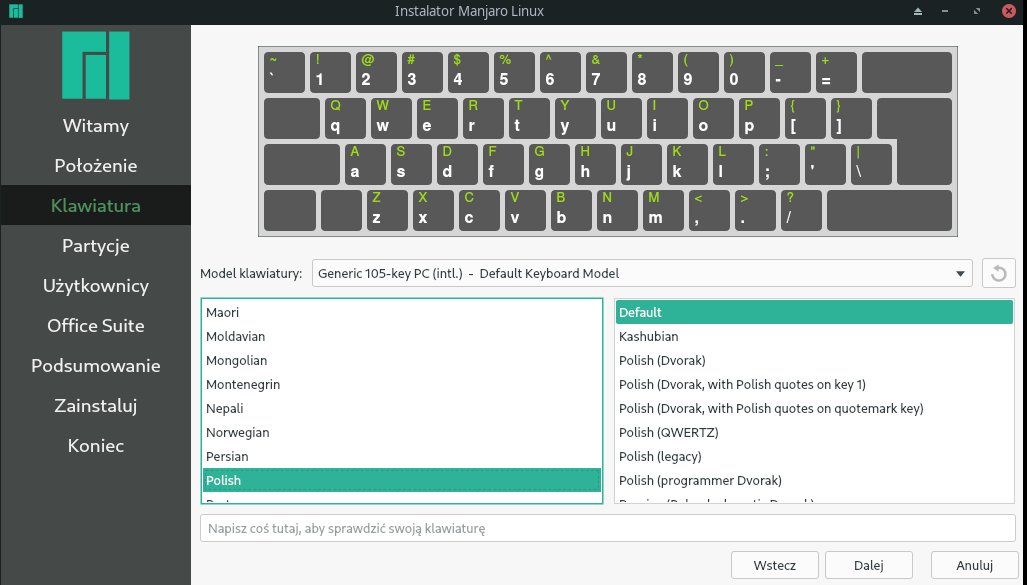
\includegraphics[width=0.95\textwidth, center]{manjaro_install5.png}\\\\\\

\item \textbf{Partycjonowanie} \par
Jest to najważniejszy etap instalacji. Tutaj czyścisz dysk aby zrobić miejsce na nowy system lub tworzysz odpowiednie środowisko z dostępnego miejsca. Dużo instalatorów posiada opcje domyślne, niewymagające własnego wkładu w partycjonowanie. Jeśli jednak nie masz takiej opcji poczytaj dokładnie poradniki do instalacji twojej dystrynbucji.\\

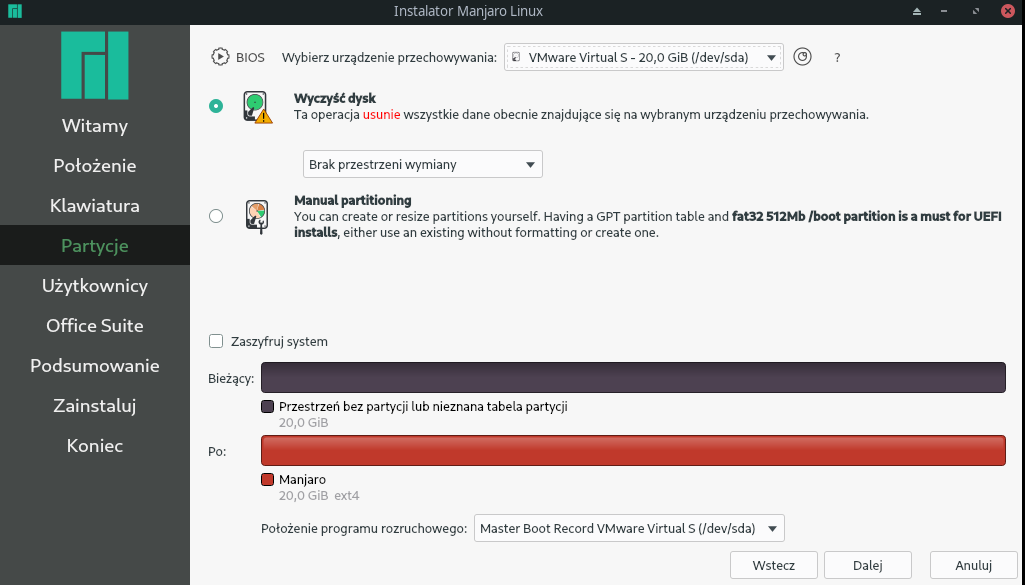
\includegraphics[width=0.95\textwidth, center]{manjaro_install6.png}\\\\\\



\item \textbf{Tworzenie kont administratora i użytkownika} \par
Aby skorzytać z systemu potrzebujemy konta umożliwiającego dostęp do niego. Podczas instalacji zawsze tworzymy konto administratora "root", które posiada wszelkie uprawnienia na maszynie. Stosunkowa większość dystrybucji wymaga utworzenia także konta upoważnionego, mającego dostęp do wykonywania operacji administratora ale posiadające inne hasło niż sam administrator. Pomaga to zwiększyć bezpieczeństwo.\\

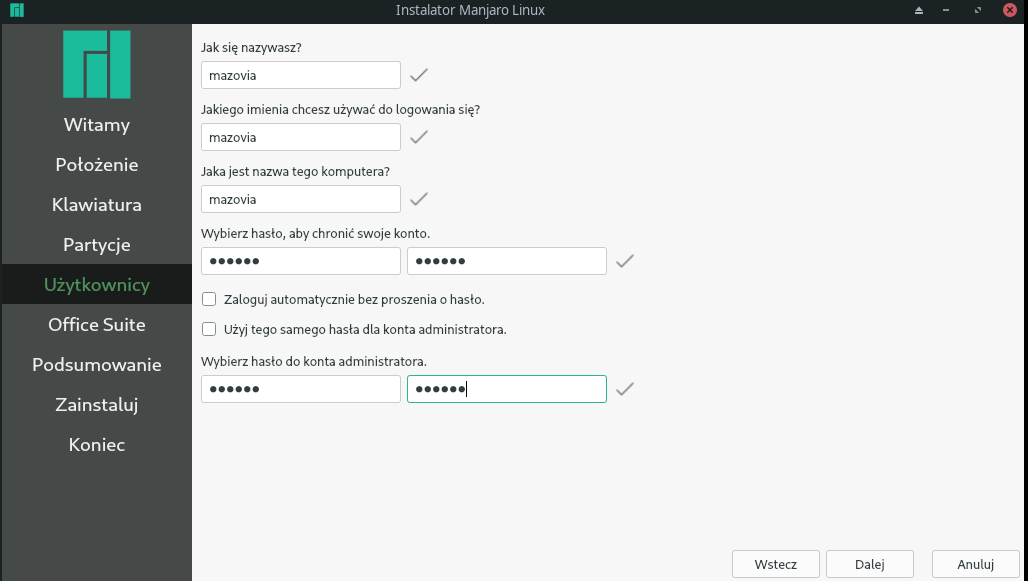
\includegraphics[width=0.95\textwidth, center]{manjaro_install7.png}\\\\\\

\item \textbf{Dodatkowe opcje} \par
Różne dystrybucje posiadają różne dodatkowe opcje poprawiające wrażenia zaraz po instalacji. Głównie dotyczą wyboru pakietów aplikacji oraz konfiguracji serwisów.\\

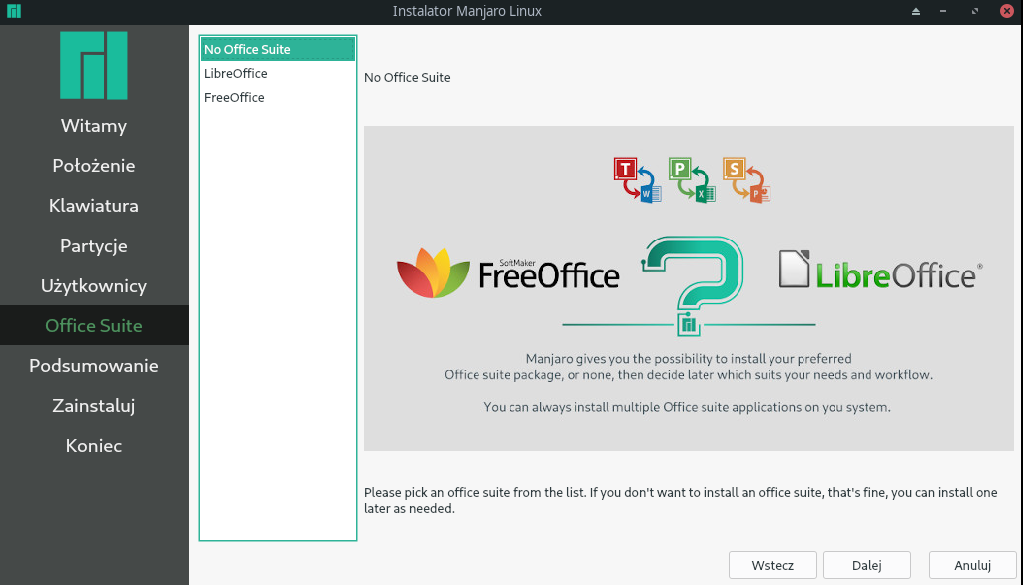
\includegraphics[width=0.95\textwidth, center]{manjaro_install8.png}\\\\\\




\item \textbf{Podsumowanie} \par
Tutaj upewnij się, że wszystkie elementy instalcji są takie same jak wybrany wcześniej. Po uruchomiueniu instalatora nie będzie można dokonać żadnych zmian. Wiąże się to też z utratą danych na dysku wiec upewnij się, że masz kopię zapasową plików ważnych dla ciebie. Jeśli jednak po instalcji okaże się, że wybrana opcja była inna niż zamierzana, a dotyczy ona samego systemu operacyjnego to po prostu uruchom instalator ponownie, tym razem wybierając odpowiednio.\\

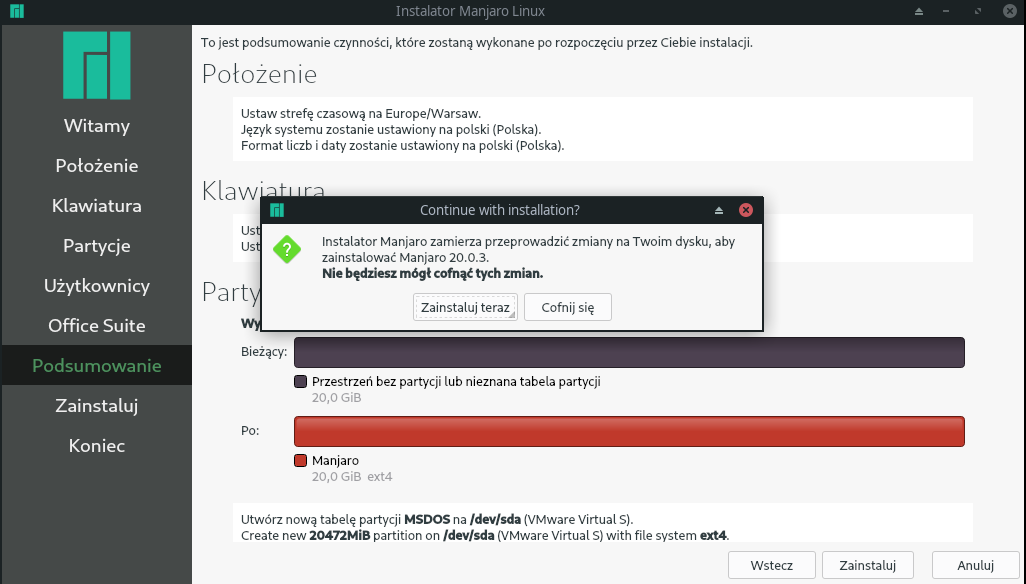
\includegraphics[width=0.9\textwidth, center]{manjaro_install11.png}\\\\

\item \textbf{Zakończenie} \par
Gdy już udało ci się poprawnie zainstalować Linuxa musisz uruchomić komputer ponownie, żeby móc korzytać z nowego systemu. Pamiętaj, że przed uruchomieniem się komputera warto wyjąć pendriva. Ułatwia to maszynie rozpoznanie dysku zawierającego system.\\

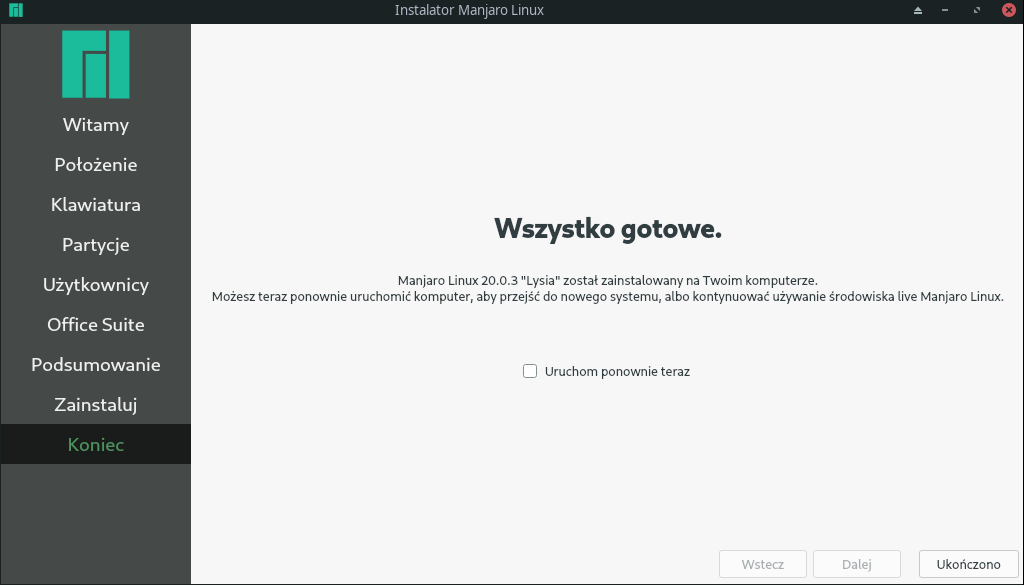
\includegraphics[width=0.9\textwidth, center]{manjaro_install13.png}\\\\\\

\end{enumerate}
 
\subsection{Konfiguracja poinstalacyjna}	

Nie każda dystrybucja jest gotowa do użytku zaraz po zainstalowaniu, a nawet te które są wciąż posiadają swoje mankamenty i małe rzeczy poprawiające wrażenia. Aby znaleźć listę takich rzeczy po prostu wyszukaj "[twoja dystrybucja] post install". Jednak jeśli nie chcesz marnować czasu na szykanie informacji przedstawiam tutaj parę najważniejszych ustawień wartych uwagi.

\begin{enumerate}

\item \textbf{Zaktualizuj system} \par Aby mieć pewność, że system jest w swojej najnowszej wersji warto zaraz po instalacji wykonać sprawdzenie aktualizacji przy pomocy wbudowanego programu. Możesz także wpisać komendy wykonujące wszystko za ciebie
\begin{itemize}
\item \textbf{Rodzina Debiana i Ubuntu} (menager pakietów APT) - \textsl{\underline{sudo apt update \&\& sudo apt upgrade -y}}
\item \textbf{Arch oraz Manjaro} (menager pakietów Pacman) - \textsl{\underline{sudo pacman -Syyu}}\\
\end{itemize}

\item \textbf{Zainstaluj sterowniki}\par Upewnij się, że wszystkie sterowniki są zainstalowane w swojej najnowszej wersji. Ich brak może wiązać się z dużymi problemami z konkretnym urządzeniem. Zapewnia to też najlepszą wydajność i stabilność.\\

\item \textbf{Zainstaluj kodeki multimedialne} Aby móc odtwarzać najróżniejsze formaty wideo i audio warto zainstalować kodeki odpowiadające za ich przetwarzanie. Można tego dokonać tą komendą choć na twoim systemie może się różnić:
\begin{itemize}
\item \textsl{\underline{sudo apt-get install ubuntu-restricted-extras}}\\
\end{itemize}

\item \textbf{Zarządzanie baterią} \par Najważniejsza opcja dla użytkowników laptopów to zestaw narędzi do zarządzania energią. Pakiet najbardziej rozbudowany i naczęściej używany to \textbf{TLP}. Pozwala znacząco poprawić żywotność laptopa oraz monitorować pobór mocy. Można go zainstalować komendą:
\begin{itemize}
\item \textsl{\underline{sudo apt install tlp tlp-rdw \&\& sudo tlp start}}\par
\end{itemize}
Aby zapoznać się z wszystkimi aspektami tego usprawnienia warto przeczytać dokumentację twórców:\\\url{https://linrunner.de/tlp/introduction.html}\\

\item \textbf{Zmniejszenie preferencji użycia pliku wymiany}\par Jeśli twoja maszyna ma powyżej 4 GB ramu to może się okazać, że system nie jest tak szybki jak mógłby być. Związane jest to z względnie agresywnym ustawienium użycia pliku wymiany zamiast pamięci RAM. Aby zapewnić szybsze działanie wystarczy zmienić wartość tej preferecji w plikach konfiguracyjnych takimi komendami:
\begin{itemize}
\item \textsl{\underline{sudo sysctl vm.swappiness=10}}\\\\\\\\
\end{itemize}

\end{enumerate}

\end{document}